\begin{figure*}
  \centering
  \begin{subfigure}[b]{\textwidth}
    \centering
    % \begin{noindent}
    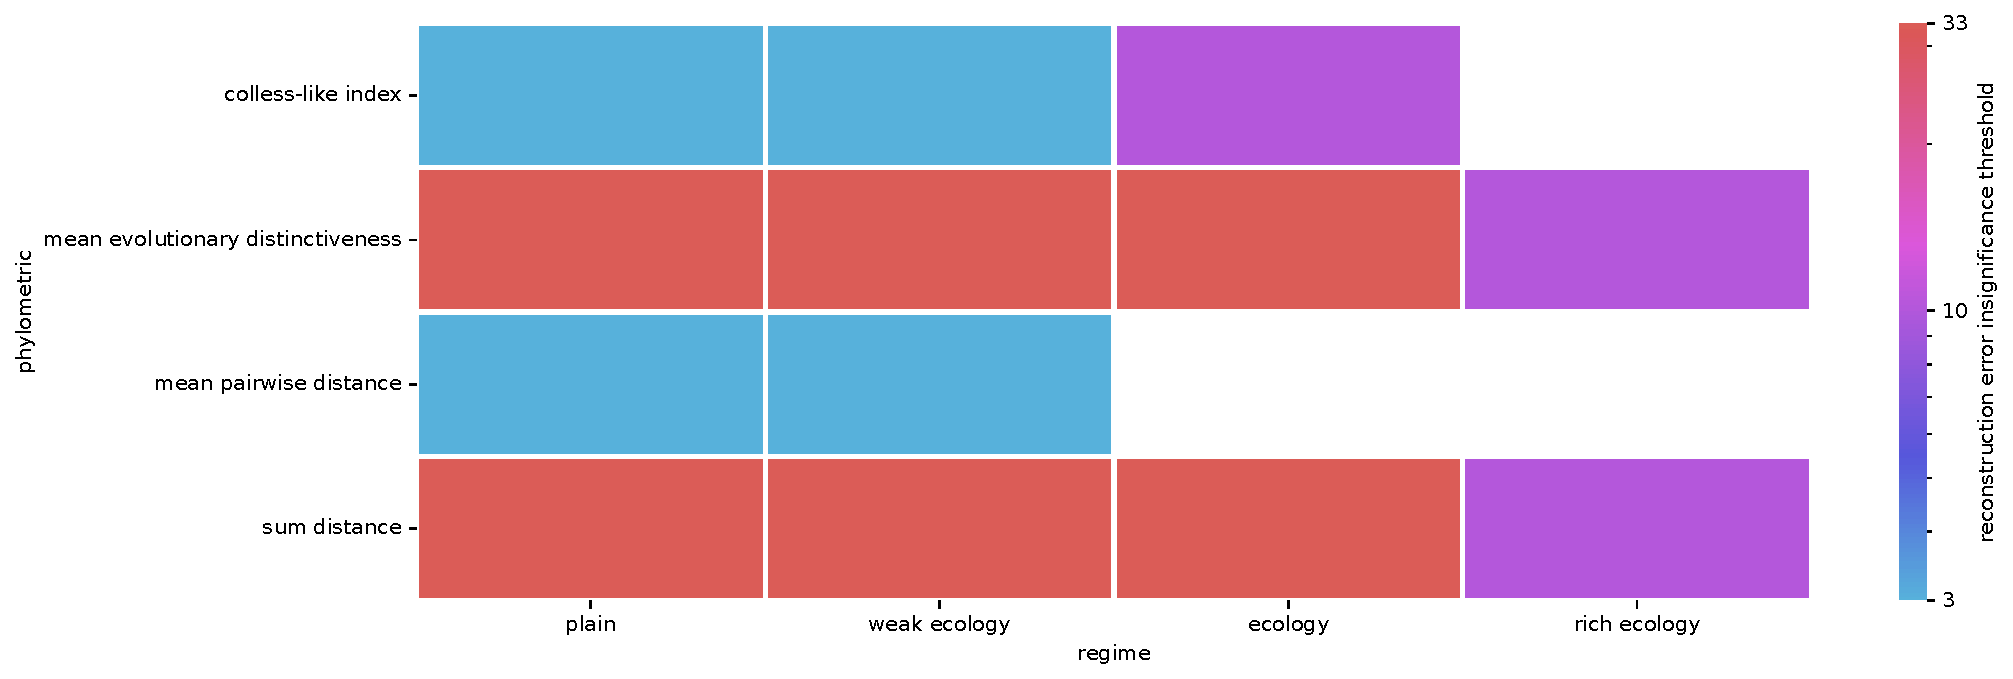
\includegraphics[width=\textwidth]{binder/binder/teeplots/epoch=0+hue=quality-threshold+mut_distn=np.random.standard_normal+nuisance=spatial-structure+viz=heatmap+x=regime+y=phylometric+ext=.pdf}
    \caption{%
      gaussian mutation distribution at epoch 0 (generation 32,768)}
    \label{fig:reconstructed-tree-phylometrics-error-spatial-nuisance-sensitivity-analysis:epoch0}
    % \end{noindent}
  \end{subfigure}
  \begin{subfigure}[b]{\textwidth}
    \centering
    % \begin{noindent}
    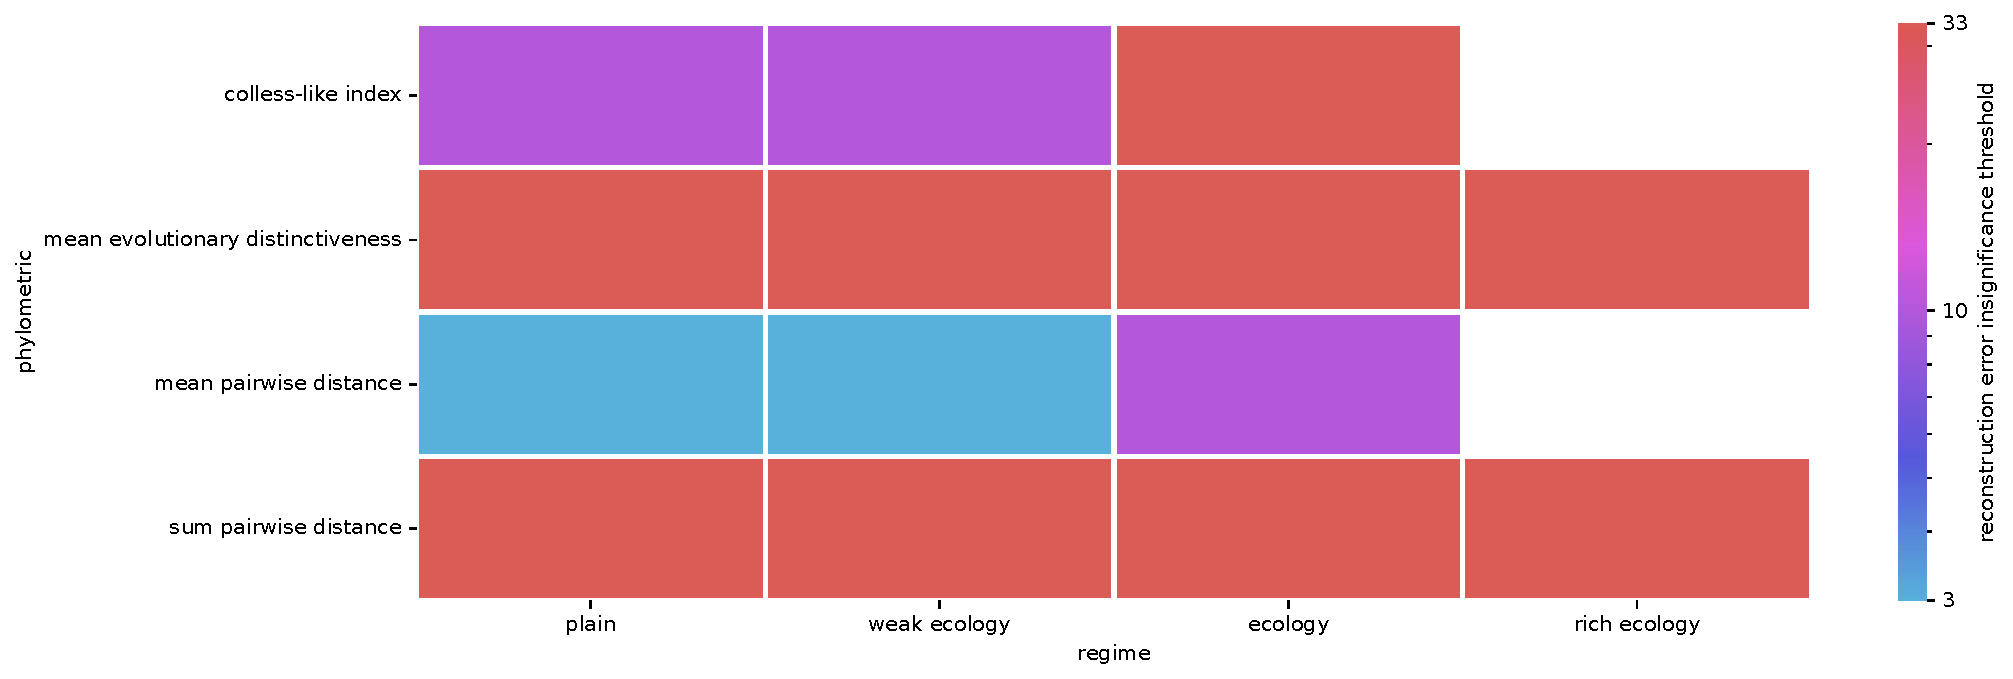
\includegraphics[width=\textwidth]{binder/binder/teeplots/epoch=2+hue=quality-threshold+mut_distn=np.random.standard_normal+nuisance=spatial-structure+viz=heatmap+x=regime+y=phylometric+ext=.pdf}
    \caption{%
      gaussian mutation distribution at epoch 2 (generation 98,304)}
    \label{fig:reconstructed-tree-phylometrics-error-spatial-nuisance-sensitivity-analysis:epoch2}
    % \end{noindent}
  \end{subfigure}
  \begin{subfigure}[b]{\textwidth}
    \centering
    % \begin{noindent}
    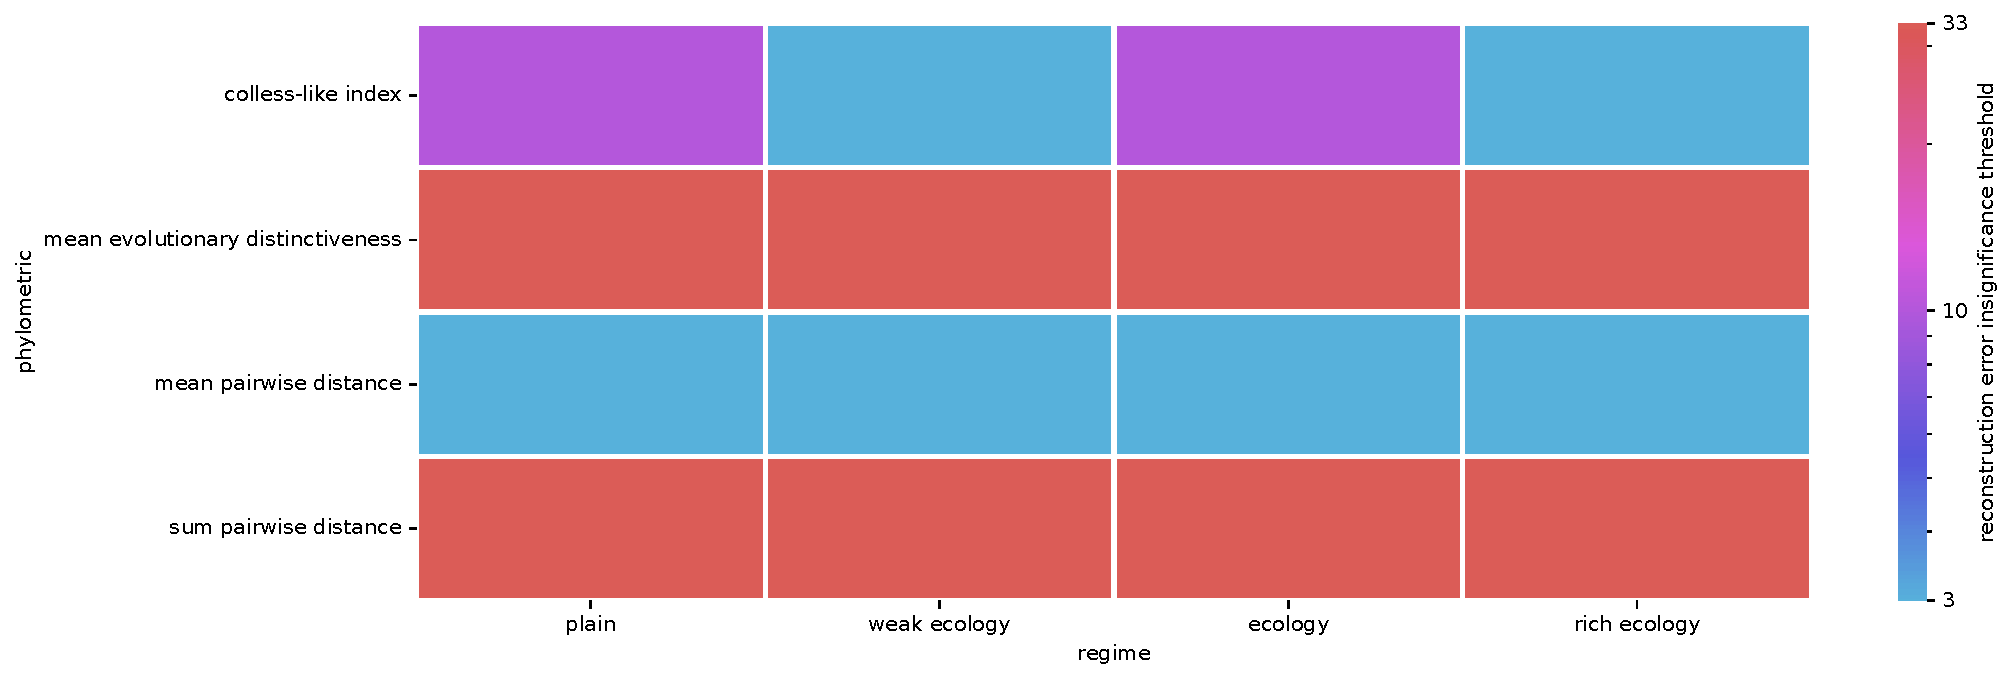
\includegraphics[width=\textwidth]{binder/binder/teeplots/epoch=7+hue=quality-threshold+mut_distn=np.random.exponential+nuisance=spatial-structure+viz=heatmap+x=regime+y=phylometric+ext=.pdf}
    \caption{%
    exponential mutation distribution at epoch 7 (generation 262,144)}
    \label{fig:reconstructed-tree-phylometrics-error-spatial-nuisance-sensitivity-analysis:exponential}
    % \end{noindent}
  \end{subfigure}
  \caption{%
    Sensitivity analysis results for reconstruction resolutions required to achieve statistical indistinguishability between reconstructions corresponding reference trees for each phylometric across surveyed evolutionary conditions with spatial structure (i.e., island count 1,024).
    Significance level $p<0.05$ under the Wilcoxon signed-rank test between samples of 50 replicates each is used as the threshold for statistical distinguishability.
    Phylometrics with looser reconstruction resolution thresholds (i.e., higher resolution percentages) are less sensitive to reconstruction error.
    White heat map tiles indicate that no surveyed reconstruction resolution threshold was sufficient to achieve indistinguishability from the reference tree with respect a particular phylometric.
  }
  \label{fig:reconstructed-tree-phylometrics-error-spatial-nuisance-sensitivity-analysis}
\end{figure*}
